\chapter{Appliance Recognition }

Appliance recognition and load disaggregation is some of the key aspects in non intrusive load monitoring (NILM). The main purpose of the NILM approach is to better understand the power usage in home, and help the different household to more optimal power savings. This is done by informing the residents about the power consumption of individual appliances. It is shown that informing a household about its usages pattern can lead to savings \fxnote{find a ref for this}. This makes the basis for load disaggregation, where appliance specific load is guessed based on the main meter load. This enables the user to know what uses the energy and when.

One other aspect of NILM is event detection. Sometime the actual consumption of an appliance is not as important as when it was used, and for how long. This is a simpler task than guessing the true consumption, and is for some applications a better approach. As an example is this kind of information sufficient if we want to track the activity of a elderly person in a assisted living situation \fxnote{find a ref for this}. 

\section{NILM Concepts And Challenges} 
The aim of NILM is to partition the hole house consumption data in to appliance specific consumption. 
\begin{equation}
	P(t) = p_1(t) + p_2(t) + ... + p_n(t)
	\label{EQ:PAC}
\end{equation}
This can be seen as in equation \ref{EQ:PAC} where $P(t)$ is the total consumption at time $t$, and $p_n(t)$ is the consumption of appliance $n$ at time $t$. The aim is to partition $P(t)$ back to the different appliance specific consumptions. In order to structure the problem we categorise the appliances in 3 groups \fxnote{ref her til a}: 

\begin{tabularx}{\linewidth}{ r X }
Type-I:&Appliances that only have 2 states corresponding to on/off. This could be a lamp or a water boiler. \\
\\
Type-II:&These are appliances with multiple states, and can be modelled as a finite state machine. Many modern devices such as TV's, computers and washing machines fall in this category.   \\
\end{tabularx}

\begin{tabularx}{\linewidth}{ r X }
Type-III:&These are appliances is referred to as Continuously Variable
Devices. These devices have a variable power draw and is impossible to model as a finite state machine. This could be appliances like power drills, and dimmer lights. These are by far the hardest for the NILM algorithms to detect. \\
\\
Type-IV:& These are a special kind of appliances that are always on and consume energy at a constant rate. Such devices could be smoke detectors and TV receivers.  \\
\end{tabularx}

Some of the different appliance types is illustrated on figure \ref{fig:ATO}. 


\begin{figure}[H]
\centering
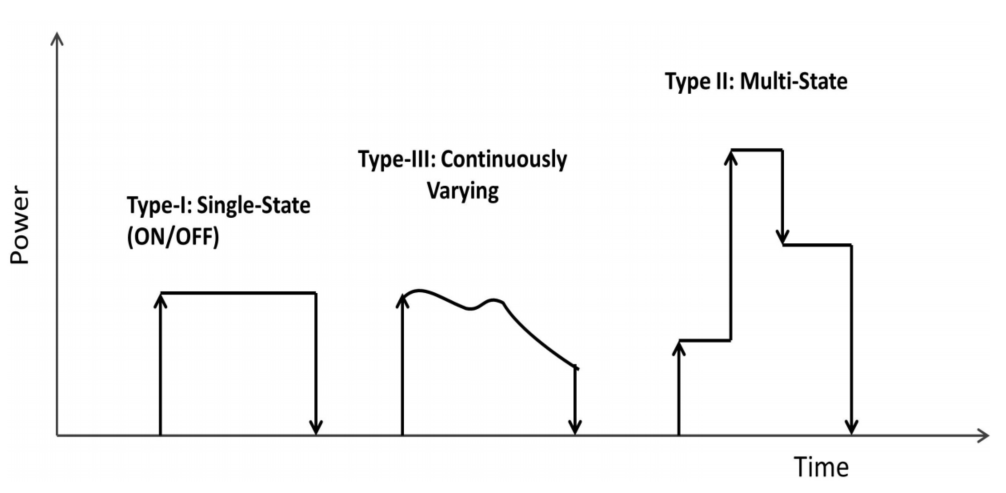
\includegraphics[width=0.6\textwidth]{billeder/Types.png}
\caption{Appliance types. Source \citep{RefWorks:17}}
\label{fig:ATO}
\end{figure}

The appliances in Type-IV is not a particular researched area, since it does not give the user much information to calculate savings from. These appliances is often using very little energy, and must not be turn off at will. 

Type-I and Type-II are very used, and can cover all most any appliance. In the area of event detection are the most common approach to see all appliances as Type-I appliances and detecting on/off events. Most appliances today is Type-II appliances due to growing amount of complicated electronics that are embedded in them. Then there are devices that are Type-II but most of the time act like Type-I appliances. An example of this is the vacuum cleaner. On most vacuum cleaners you are able to change the suction intensity, which makes it type two. But most people don't change this very often, so the energy usage looks more like a Type-I appliance. 
 
\subsection{NILM Features} 
For data disaggregation it is common to use method based in machine learning and optimization. The approach is to first extract features from the dataset, and then train or validate by using this features. 

In NILM the features can be sub categorised in steady state, transient state and non-Traditional features.  These categories can be further expanded as shown on figure \ref{fig:FTR}. 

\begin{figure}[H]
\centering
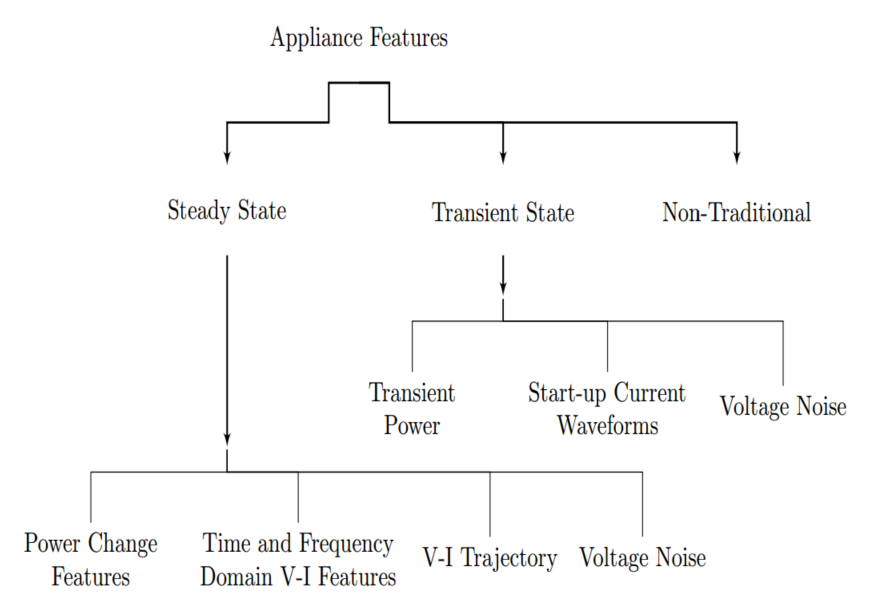
\includegraphics[width=0.6\textwidth]{billeder/featureOverview.png}
\caption{Feature types. Source \citep{RefWorks:17}}
\label{fig:FTR}
\end{figure}

Steady state features is features that can be extracted when the signal is in the stable state. Features that are often extracted in this state is "Power Change" which is the jump in power or reactive power usage. Time and frequency analysis is often used on the voltage and power signals of the meters. It is shown that analysing the harmonics in signals is a powerful way of making appliance detection \fxnote{ref}.The trajectory between voltage and power usage is a god feature. This can be used to detect the reactive power of a signal, which is a give-away for inductive loads. Some researchers have shown that different appliances makes different noise profiles on the main line. Unfortunately does this kind of recognition require a extremely high sampling rate \fxnote{ref}. 

The transient state of an appliance is a short state that comes when a appliance switches between steady states. In this state there often is appliance semi-unique waveforms in the current and voltage domain. The noise generated on the mainline in this state is also a good indication of the appliances type. 

There also exists a series of non-traditional features, that is used in special types of algorithms. One of them is based on matching the power usage profile to geometrical figures, and using the series of figures to recognize an appliance \fxnote{ref}.  

Many of the above features requires a high sample rate in kHz or Mhz span in order to be effective. This is often not the case, since it is normal smart meters that are providing the data. For a smart meter a sample rate at 1 Hz would be considered fast, and for many applications this is down to $0.03$ Hz or slower. It is therefore common only to use the steady state features, and most of the time only the power change feature, which looks at changes in power, reactive power, current or voltage. 

\subsection{Learning Strategy} 
When you have extracted features from the signal there are several algorithms there can be selected for the training. They can roughly be split up in two categories, optimization algorithms and machine learning algorithms. The optimization algorithms relies on a database of appliance info, and tries to find the subset of the database that are most likely to be in use. 
\begin{equation}
	M = \argmin_{x \in \powerset{D} } \left( \mid {\sum_{i = 0}^{I} x_i - \hat{y}  \mid} \right)
	\label{EQ:OMP}
\end{equation}

This is illustrated in equation \ref{EQ:OMP} were a set of appliances $M$ that correspond to the measured signal $\hat{y}$. This is done by searching the known database of all appliances $D$. This is done by taking the power set of the database and find the subset that fits best. 

This approach is fine for a small amounts of appliances, but for large databases and many appliances in use at the same time, does this take far to long to be practical. 

Many uses therefore the machine learning techniques, to get results that are faster and scale better. There are two main categories of machine learning: supervised and unsupervised. 



%	-- Learning metoder

% 	-- Signaler der drukner i andre

\section{Related Work} 

%	-- NILMTK 
%	- Neural net 
			

\section{Recognition Methods} 


\section{The ECO Dataset} 

\section{Validation of Methods} 